\documentclass[a4paper,11pt]{article}
\usepackage[utf8]{inputenc}
\usepackage{amsmath}
\usepackage{amsfonts}
\usepackage{amssymb}
\usepackage{graphicx}
\usepackage{braket}

\numberwithin{equation}{section}
\renewcommand\thesubsection{\alph{subsection}}
\newcommand{\bvp}[1]{\mathbf{#1}'}
\newcommand{\bv}[1]{\mathbf{#1}}
\newcommand{\ez}{\epsilon_0}
\newcommand{\eo}{\epsilon_1}
\newcommand{\lrp}[1]{\left({#1}\right)}
\newcommand{\lrb}[1]{\left\{{#1}\right\}}


%opening
\title{Computational Biophysics HW6}
\author{Vince Baker}

\begin{document}

\maketitle

\section{Q1}
We first find the coefficients as $\gamma\Delta t \rightarrow 0$.
$c_0$ clearly approaches 1, and $c_1$ approaches 1 by L'Hopital's rule.
Expanding $c_2$ in terms of $x \equiv \gamma\Delta t$ and using L'Hopital's rule twice we find:
\begin{align}
 c_2 &= \lrp{\frac{1}{x}\lrp{1-\frac{1}{x}+\frac{e^{-x}}{x}}}|_{x\rightarrow 0}\\
 c_2 &= \lrp{\frac{x+e^{-x}-1}{x^2}}|_{x\rightarrow 0}\\
 c_2 &= \lrp{\frac{1-e^{-x}}{2x}}|_{x\rightarrow 0}\\
 c_2 &= \lrp{\frac{e^{-x}}{2}}|_{x\rightarrow 0}\\
 c_2 &= \frac{1}{2}
\end{align}
$\sigma^2_v$ clearly approaches 0. 
Applying the same method above to $\sigma^2_r$ and ignoring the constants in front:
\begin{align}
 \sigma^2_r &= \frac{1}{x}\lrp{2-\frac{1}{x}(3-4e^{-x}+e^{-2x})}|_{x\rightarrow 0}\\
 \sigma^2_r &= \frac{2x-3+4e^{-x}-e^{-2x}}{x^2}|_{x\rightarrow 0}\\
 \sigma^2_r &= \frac{2-4e^{-x}+2e^{-2x}}{2x}|_{x\rightarrow 0}\\
 \sigma^2_r &= \frac{4e^{-x}-4e^{-2x}}{2}|_{x\rightarrow 0}\\
 \sigma^2_r &= 0
\end{align}
A random variable drawn from a zero-mean Gaussian distribution with a variance of 0 is identically 0.
Therefore our Langevin equations reduce to:
\begin{align}
 \bv{r}(t+\delta t) &= \bv{r}(t) + v(t)\delta t + \frac{1}{2}a(t)\delta t^2\\
 \bv{t+\delta t} &= v(t) + a(t)\delta t
\end{align}
These are just the inertial equations of motion, as we could see from the demonstration in class.

\section{Q2}
Taking the extreme limit as $\gamma\Delta t\rightarrow\infty$ it is clear that $c_0,c_1$ and $c_2$ all approach 0.
$\sigma^2_r$ approaches 0, while $\sigma^2_v$ approaches $\frac{kT}{m}$. 
So the Langevin equations reduce to:
\begin{align}
 \bv{r}(t+\delta t) &= \bv{r}(t)\\
 \bv{t+\delta t} &= \Delta\bv{v}^G
\end{align}
So the particle can be modeled as having a random velocity at each point in time, with the variance of the speed being $\frac{kT}{m}$.
The motion is therefore diffusive rather than inertial, and we expect the ``random walk'' trajectories we observed in class.

\section{Q3}
Using our results from Q1, we find the limit of equations 71 and 72:
\begin{align}
 \bv{r}(t+\delta t) &= \bv{r}(t) + v(t)\delta t + \frac{1}{2}a(t)\delta t^2\\
 \bv{v}(t+\delta t) &= v(t) +\frac{1}{2}a(t)\delta t + \frac{1}{2}a(t+\delta t)\delta t\\
 \bv{v}(t+\delta t) &= v(t) +\frac{1}{2}\delta t (a(t+\delta t) +a(t)) 
\end{align}
These are the velocity Verlet equations.

\section{Experiment}
\begin{tabular}{l | c | c | c | r}
 Gamma & Slope & D & T & T/gamma \\
 \hline
 5 & 1.1543 & 0.1924 & 1.0234 & 0.2047 \\
 6 & 0.9923 & 0.1654 & 1.0331 & 0.1722 \\
 7 & 0.8108 & 0.1351 & 1.0287 & 0.1470 \\
 8 & 0.7486 & 0.1248 & 1.0301 & 0.1288 \\
 9 & 0.6443 & 0.1074 & 1.0330 & 0.1148 \\
 10 & 0.5583 & 0.0931 & 1.0390 & 0.1309 \\
 12 & 0.4909 & 0.0818 & 1.0425 & 0.0869 \\
 15 & 0.3658 & 0.0610 & 1.0514 & 0.0701 \\
 20 & 0.2714 & 0.0452 & 1.0605 & 0.0530 \\
 \hline
\end{tabular}

The diffusion coeeficient may be estimated by  $\frac{1}{6}\frac{d r^2}{dt}$, or through $D=\frac{kT}{m\gamma}$.
The diffusion coefficient estimated from the mean squared displacement is plotted against $T/\gamma$ below, and the slope of the line is 1 as expected.
\begin{figure}[h]
 \caption{Diffusion coefficient measured using alternate methods}
 \centering
   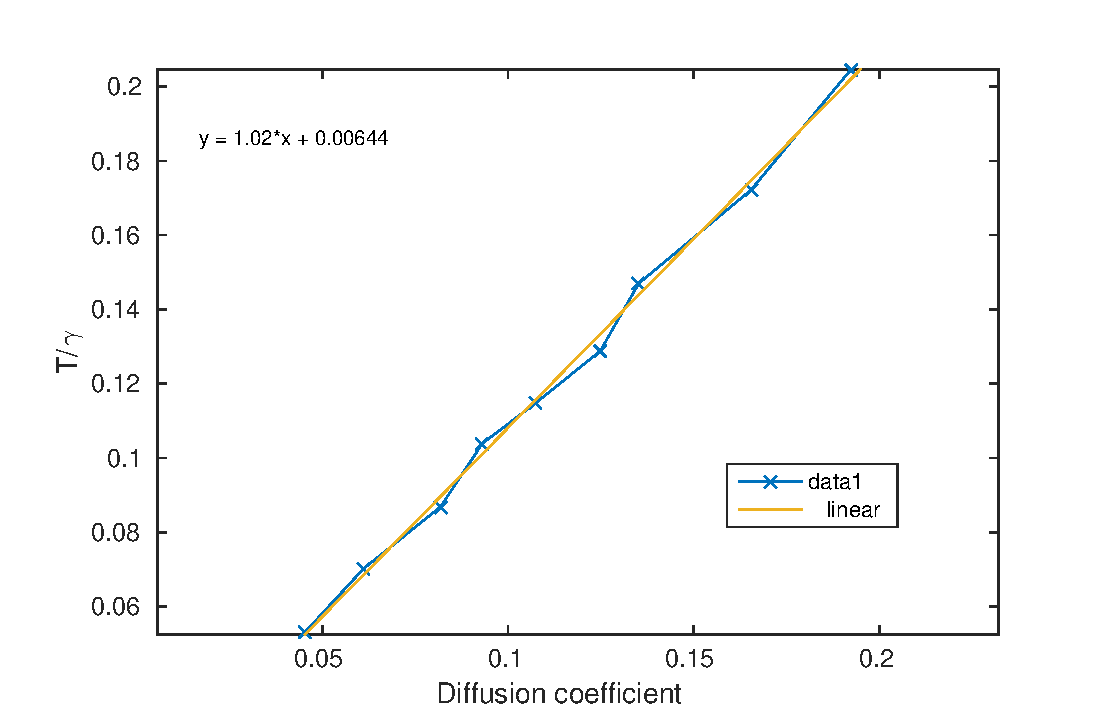
\includegraphics[width=\textwidth]{DC_vs_ty}
\end{figure}


\end{document}
